\chapter{改进从团队开始} % Introduction chapter suppressed from the table of contents

上一章介绍了丰田方式中七个水面下的习惯，那么公司如何有效地开展和推广这些理念呢？有哪些需要注意的误区？让我们从美国东海岸一家小型印刷公司的故事说起。

\hypertarget{ux7f8eux56fdux8d39ux57ceweisbordux6545ux4e8b}{%
\subsection{美国费城Weisbord故事}\label{ux7f8eux56fdux8d39ux57ceweisbordux6545ux4e8b}}

在上世纪60年代，复印机尚未普及且价格昂贵，因此有不少公司专门为各类客户提供印刷服务。故事的主角 Weisbord 是美国东岸一家印刷公司老板的儿子，他没有接受过正式的管理培训。他的好友 Don 已经在一家国际大公司工作了20年，向 Weisbord 推荐说：“很多大公司已经开始推行团队自主管理，以提高生产率。你可以先读读《X-Y 理论》（McGregor 著，Human Side of Enterprise）这本书。”\\

\textbf{X 理论：}

对(员工)人性的假定

\begin{itemize}
\tightlist
\item
  懒散 /不想工作，尽可能避开责任
\item
  依赖/被动希望被指挥，工作安稳最重要
\item
  因此主管必须要把工作细分，并要紧密管控才会达到结果
\end{itemize}

\textbf{Y 理论：}

假定

\begin{itemize}
\tightlist
\item
  关注工作，希望负责任(take responsibility)
\item
  希望成长，有成就
\item
  如给予机会，会尽力把事情做好
\end{itemize}

\hypertarget{ux95eeux9898ux5904ux4e8exux601dux7ef4ux7684ux4e3bux7ba1}{%
\subsection{处在X思维的主管}\label{ux95eeux9898ux5904ux4e8exux601dux7ef4ux7684ux4e3bux7ba1}}

Weisbord原本只是好奇，想看看这本书有多厉害，结果一个周末便一口气读完了。他意识到自己的公司到处都是X理论式的管理：

\begin{itemize}
\tightlist
\item
  工作分得很细，每个员工不清楚全局
\item
  任务都是依赖主管分配
\item
  员工遇到问题、困难，交给主管处理
\item
  员工上下班打卡
\end{itemize}

他认为新方式可以提升公司的管理，因担心自己难以推动这项改革，便正式邀请好友Don加入公司。\\
通过分析，他们发现公司业务的最大问题出在订单处理部门（Order Processing），每个订单被拆分成五到六个独立的任务，员工仅负责被分配到的任务，如：


\begin{itemize}
\tightlist
\item
  筛选客户邮寄地址，邮寄印刷样本
\item
  输入订单。
\item
  检查客户的信用
\item
  发起内部生产订单
\item
  用打字机打发票邮寄出去
\item
  收到的支票，对上那些应付账\\
\end{itemize}

公司平均每天要处理200到300个订单，但由于任务划分过细，一旦某个环节（如订单录入）有一两人缺席，便严重拖累整个流程，效率可能因此减半。\\
为解决这一问题，Weisbord计划对部门进行改革，将订单处理部门分成多个4至5人的团队，再将公司的2万个客户按地区分配给各团队。每个团队负责自己区域内的客户，并配备打字机等设备，希望以此提升部门的灵活性，提高生产效率。\\

他与五位小组主管讨论改革方案，其中两位表示支持，两位持中立态度，剩下的一位认为方案不会成功。\\
Weisbord最终决定启动这一改革，与Don一同开展部门重组的工作。


\hypertarget{ux5f00ux59cbux56e2ux961fux5236}{%
\subsubsection{开始团队制}\label{ux5f00ux59cbux56e2ux961fux5236}}

开始时问题非常多：

\begin{itemize}
\tightlist
\item
  B物流公司运送出错，送到另一个城市，怎么办
\item
  D团队误解了生产的步骤，怎么办
\item
  C团队的样板工人，刚入职3 周，对我们公司产品线不熟识，怎么办\\
\end{itemize}

原因很简单：原来每人只熟悉自己负责的一小块工作，遇到问题都由小主管处理。而在自主团队中，没有主管的支持，每个团队都需自行解决问题，感觉就像瞎子摸象。\\
但问题确实太多了，无奈之下，Don建议每周开会讨论，但团队从来没有定期会议的习惯。起初，Weisbord认为开会浪费时间，不如把时间用于生产更实际些。然而，问题依然层出不穷，这种情况延续了一个月。\\
Weisbord开始对X-Y理论产生怀疑，觉得这些理论可能只适合在象牙塔，而难以在实际公司运作中落地。Don也无更好的应对策略，Weisbord甚至萌生了放弃改革、恢复原有架构的念头。尽管Don建议再耐心等待一两周，Weisbord因团队持续的效率低下、公司运作受到影响，打算在下次会议上宣布撤销改革。\\

到了第五周，与以前开会一样，Weisbord先问: 大家有什么问题？\\
会议室一片沉默。几分钟后，一位组长说道：“没有问题。”\\
Weisbord感到惊讶：“怎么会没有？之前一直问题不断。”（心里想，一定是你们也放弃了，连问题都不愿提了。）\\
另一位组长回答：“本周我们确实没有什么问题，因为遇到的问题在之前会议里解决了。”\\

\hypertarget{ux6548ux679c}{%
\subsubsection{效果}\label{ux6548ux679c}}

改革最终带来了显著成果：每天的订单处理量从不足300单提升至400单，员工的出勤率也显著改善，缺席率几乎为零。\\
改革后的订单处理部平面图：

%\href{文件:0A_Agile_stories_p5.jpg}{文件:0A Agile stories p5.jpg}

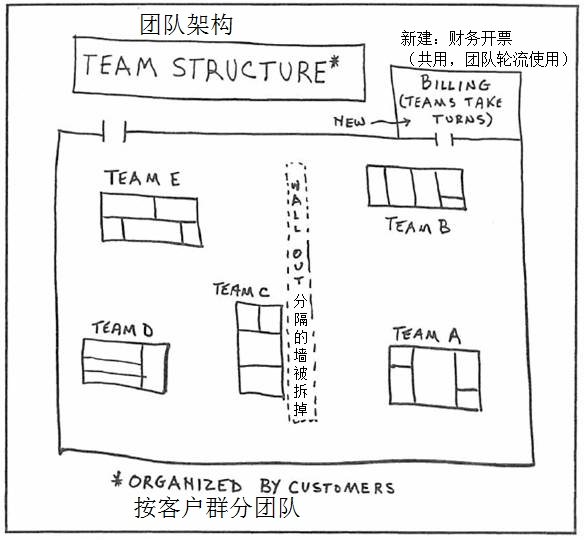
\includegraphics[width=10cm]{0A_Agile_stories_p51.jpg}

（在团队改革前，小主管们为减少在处理订单时的摩擦，曾在部门内加了一道隔墙，到后来团队一致认为拆除隔墙更有助于沟通协作）\\
Weisbord事后总结道：任何变革和重组都需要时间来磨合，期间管理者的持续支持至关重要。如果管理者不能坚持到底，直面并解决遇到的困难，改革很容易半途而废。\\

\hypertarget{ux542fux53d1}{%
\subsection{启发}\label{ux542fux53d1}}

如果员工具备知识技能，管理者便应尽力给员工平台，让团队自主发挥，才能不断提升竞争力，应对变化万千的市场需要，让员工与公司都受益。管理者不仅仅是制订目标、计划，发号施令的角色，而更应该是一位导师，辅助团队成长。\\
这故事也引出推行丰田式改善的4个常见误区：

\begin{itemize}
\tightlist
\item
  不要指望一蹴而就
\item
  只能坚持到有结果，不能半途而废
\end{itemize}

\begin{description}
\tightlist
\item[]
本来Weisbord和Don误以为会很快就有效果，预估不了会出现这么多问题，如果他们没有坚持到底，就会以失败告终。
\end{description}

\begin{itemize}
\tightlist
\item
  最重要是培养人才，但训练比教育更重要
\end{itemize}

\begin{description}
\tightlist
\item[]
大野先生认为：教育式教对方他们本来不知道的东西。训练是让对方重复练习已经知道的东西，让他们牢牢记住该怎样做。要做好训练，领导或内部教练必须能够身先士卒带头动手做。不然会容易被批``光会嘴巴说，但什么都不干''。
\end{description}

\begin{itemize}
\tightlist
\item
  让员工自己找答案
\end{itemize}

过程改进需要每一个部门都参与，要由团队自己去找答案，而不是直接告诉他们怎么做，才可以提升公司的最终目标，

大部分已经是九零后了，很多员工都有自己的想法，很难要求他们像以前只听从主管指挥。所以也不能再依赖专家（外部或内部）和顾问解决问题，必须所有员工参与改进整个系统。上面费城故事就是领导让团队记住自主和学习，完成订单处理部门从传统主管式管理改组成团队自主管理的例子。当时，改成团队制后开始每周开会，不仅仅解决团队的疑问，其实也促进团队之间的交流，了解其他团队的问题。如果管理层认同这种新的管理模式，组织架构从本来的功能划分变为小组独立自主管理外，还有什么具体方法促进公司走向？所有员工参与改进整个系统？


\begin{description}
\tightlist
\item[]
回顾过去，放眼未来
\end{description}

最后依据培训的主题，让大家讨论并制定具体的改进目标和行动计划。

但若要有效果，管理者必须定期监控：

\begin{description}
\tightlist
\item[]
改进效果如何

遇到什么困难计划

计划要不要调整
\end{description}

若不及时监控，团队会觉得只是一般的培训，学完便完事了。

工作坊可以促进团队间的了解，例如：

\begin{itemize}
\tightlist
\item
  产品开发部原来不知道现场实施工程师对新产品的安装和使用还是有很多误解。

  \begin{itemize}
  \tightlist
  \item
    后面开发部除了做安装手册也录视频，减少现场工程师误解。
  \end{itemize}
\item
  开发工程师从现场实施工程师了解到有些因为现场测试不通过，导致不能按时发新版本的主因。

  \begin{itemize}
  \tightlist
  \item
    原来客户验收有一套标准的流程，包括他们的测试数据和步骤，但测试人员交付前的检测都只是按自己理解测试，与客户验收流程有出入。
  \end{itemize}
\end{itemize}

\hypertarget{ux82acux5170ux8ba1ux5212}{%
\subsection{芬兰计划}\label{ux82acux5170ux8ba1ux5212}}

要具备什么条件才能让敏捷开发团队有好成绩？

再邀请你来听我讲ACP的第一堂课。

\begin{description}
\item[]
\begin{description}
\tightlist
\item[]
(ACP = Agile Certified Professional 是美国 PMI 推的敏捷管理个人资质。）
\end{description}
\end{description}

%\href{文件:GoogleVsYahoo_Screenshot_2024-10-24_132145.jpg}{600px}

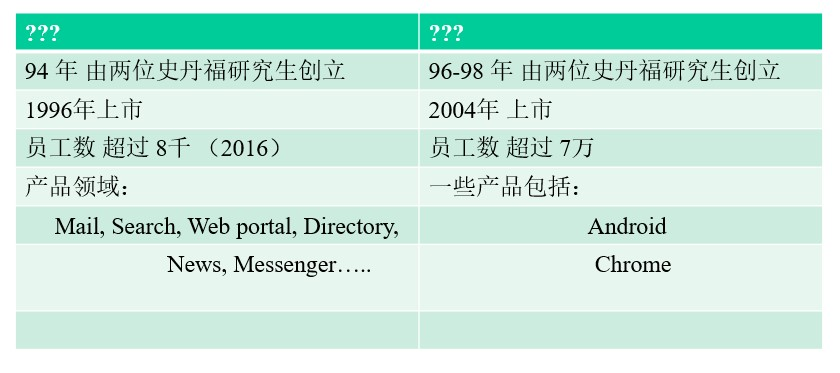
\includegraphics[width=10cm]{GoogleVsYahoo_Screenshot_2024-10-24_132145.jpg}

表2-1

``请问大家左右两家美国西岸IT公司是什么公司？''\\
估计你们都能猜到右面的是谷歌Google，但不一定能认出左面的是Yahoo！因为后者在2016年已经被收购。在2001年时，谷歌是刚成立不久的小公司，雅虎是首批互联网公司，当时已经是有名的上市大公司，市值比福特、通用汽车公司还高，并不断收购公司扩大业务。但也养成了很多``大公司''病------官僚化管理。例如很多决策或改进都需要管理层多层审批，有很多X管理的味道。\\
谷歌(Google)公司是由两位史丹福大学研究生Larry Page ，ergey
Brin创办。在2000年,Eric
Schmidt加入并担任CEO（他之前是Novell的CEO，以前在SUN
Microsystems工作）,Jonathan
Rosenberg也加入并出任产品经理（他之前在Apple当产品经理）。\\
谷歌的管理很扁平，当Eric
Schmidt第一天进公司当CEO，他本来是Novell的CEO。因为谷歌公司快速发展员工很多，办公空位不够，人事部经理好不容易才为他找到一个办公室，但过了几天有一位工程师来问：``我那边的办公地点是在太剂了，我看你的办公室应该还可以容立多一个人。我可否搬过来过来？''\\
虽然Eric Schmidt觉得很奇怪，但因为刚进公司，就接受了。\\
当时谷歌(Google)还是很小的公司,但因在搜索引擎上有所突破，
预计会被微软攻击和收购。董事会主席Mike Moritz 便请刚进公司的CEO
Eric和产品经理Jonathan准备了一份详细的商业计划书来应对，代号``芬兰计划''。俩人经过两个多月细心准备，约创始人Larry开会解释计划详细内容，Larry拿到计划书快速看了一下，便立马问他们俩：``你们以往有试过超出你们的计划吗？
如果没有，建议还是先跟我们那些工程师聊聊吧。''\\
后面他们俩发现Google的工程师都是精英，无论技术或业务方面的能力都很强，都有很多创新思路。了解到如果还是按传统的计划驱动反而会限制团队的创新能力。\\
Eric与Jonathan后面把谷歌的独特文化写成书 ``How Google
Works''，他们把公司里这些优秀人才统称为聪明创意人(Smart Creatives)。\\
当我讲到这里时，便把书的目录派给学员，然后讲解书里相关章节，介绍谷歌公司文化：

\hypertarget{ux4e03ux7684ux89c4ux5219the-rule-of-seven}{%
\subsubsection{七的规则(The Rule of
Seven)}\label{ux4e03ux7684ux89c4ux5219the-rule-of-seven}}

一般公司组织架构都会限制主管直属下属人数，谷歌当时也规定人数为7，但规定直接下属不能少于7，可以看到他们组织架构多扁平。

\hypertarget{ux6cb3ux9a6c-hippo}{%
\subsubsection{河马 HiPPO}\label{ux6cb3ux9a6c-hippo}}

河马(Hippopotamuses)是攻击力很强，非常危险的动物。\\
谷歌公司用河马的英文简称 HiPPO (Highest Paid Person's
Opinion)，比喻企业类内的"大王"按自己的主观判断，雷厉风行也是非常危险。\\
例如在谷歌的内部讨论会，做决定不看提出意见者在公司的地位、权威。高管提出的建议，如果缺乏充足的数据支持，也可以被工程师推翻，例如创始人之一Sergey想某工程部协助开发某新产品，但他的方案缺乏有力数据支撑，工程主管不同意。Sergey没有用他的权威强制要求（他绝对有这权力），他让步妥协，只需要一半人手参与，但工程主管还是不同意，最终大家客观比较各种方案的优劣，Sergey的方案未被采纳。

\framebox{%
\begin{minipage}[t]{0.97\columnwidth}\raggedright
谷歌有个特点，每次开会都会用2个投影仪，其中一个是专门投放数据的。很多公司管理层都会嘴巴说用数据说话。
\strut
\end{minipage}}

\hypertarget{ux4e24ux4e2aux62abux8428ux7684ux89c4ux5219bezos-two-pizza-rule}{%
\subsubsection{两个披萨的规则(Bezo's two pizza
rule)}\label{ux4e24ux4e2aux62abux8428ux7684ux89c4ux5219bezos-two-pizza-rule}}

两个披萨应该让团队够吃，团队人数不能太多，妨碍有效沟通。

\hypertarget{ux5458ux5de5ux5de5ux4f5cux996eux98dfux751fux6d3bux5728ux4e00ux8d77work-eat-live-together.keep-them-crowded}{%
\subsubsection{员工工作饮食生活在一起(Work, eat, live together.),(Keep
them
crowded)}\label{ux5458ux5de5ux5de5ux4f5cux996eux98dfux751fux6d3bux5728ux4e00ux8d77work-eat-live-together.keep-them-crowded}}

这跟敏捷开发要求团队必须面对面沟通，一起工作，效率才会高如出一辙。

\hypertarget{ux6240ux6709ux91cdux7ec4ux5728ux4e00ux5929ux5185ux5b8cux6210do-all-reorgs-in-a-day}{%
\subsubsection{所有重组在一天内完成(Do all reorgs in a
day)}\label{ux6240ux6709ux91cdux7ec4ux5728ux4e00ux5929ux5185ux5b8cux6210do-all-reorgs-in-a-day}}

因为市场变化快，组织必须频繁重组才能跟上。为了减少重组对工作的影响，规定每次重组必须快速完成。

\hypertarget{ux9488ux5bf9ux5ba2ux6237focus-on-the-user}{%
\subsubsection{针对客户(Focus on the
user)}\label{ux9488ux5bf9ux5ba2ux6237focus-on-the-user}}

\hypertarget{ux5236ux5b9aux51e0ux4e4eux8fbeux4e0dux5230ux7684ux76eeux6807set-almost-unattainable-goals}{%
\subsubsection{制定几乎达不到的目标(Set \{almost\} unattainable
goals)}\label{ux5236ux5b9aux51e0ux4e4eux8fbeux4e0dux5230ux7684ux76eeux6807set-almost-unattainable-goals}}

这2条与前面丰田的文化类似。也验证了持续改善的原则不仅适用于制造业。

\hypertarget{ux89c4ux5219}{%
\subsubsection{70/20/10规则}\label{ux89c4ux5219}}

\begin{itemize}
\tightlist
\item
  70\%的时间用于和核心业务
\item
  20\%用于具备潜力的新产品
\item
  10\%是用于全新的产品（例如在初步构思阶段）
\end{itemize}

\hypertarget{ux89c4ux5219-1}{%
\subsubsection{20\% 规则}\label{ux89c4ux5219-1}}

员工都可以用20\%的时间用于自己有兴趣的项目。\\
以前惠普公司（创始人Hewlett和Packard本身都是工程师）也规定公司实验室七天24小时开放。欢迎工程师任何时间进实验室做自己感兴趣的项目，不一定局限于公司安排的项目。很多创新的产品不是高层可以通过想象得出来的。\\
例如谷歌的Android，就是其中一个员工特别喜欢玩手机操作系统，开始的时候，他是用自己时间创建出来，后面成为谷歌产品的其中一条主力。

\hypertarget{ux5982ux9879ux76eeux4e0dux80fdux8fbeux5230ux9884ux671fux6548ux679cux4fbfux7acbux9a6cux53ebux505cfail-well}{%
\subsubsection{如项目不能达到预期效果，便立马叫停(Fail
well)}\label{ux5982ux9879ux76eeux4e0dux80fdux8fbeux5230ux9884ux671fux6548ux679cux4fbfux7acbux9a6cux53ebux505cfail-well}}

例如谷歌Sydney分公司推出新一代电子邮箱服务，虽然里面有很多创新，但一直没有达到预期的用户数量。便被叫停。

\hypertarget{ux9891ux7e41ux4ea4ux4ed8ux548cux8fedux4ee3ship-and-iterate}{%
\subsubsection{频繁交付和迭代(Ship and
iterate)}\label{ux9891ux7e41ux4ea4ux4ed8ux548cux8fedux4ee3ship-and-iterate}}

因为市场和需求快速变化，企业必须跟上节奏，尽量减少浪费。\\
这条与上一条类似，都是精益和敏捷开发的原则。

\begin{description}
\item[]
\begin{description}
\tightlist
\item[]
=== === ===
\end{description}
\end{description}

2000年时，谷歌在快速成长期。我通常会在敏捷培训课的第一天借用谷歌的故事说明团队敏捷开发的成败依赖于公司文化。

\framebox{%
\begin{minipage}[t]{0.97\columnwidth}\raggedright
讲敏捷课时，某学员听完敏捷精益的概念后，说她的经理要求她输出一份3个月的详细工作任务分解，且要求活动的颗粒度细到5天之内，因为她的经理按计划管理的思路很重。她很困惑，软件开发变化这么多，怎么可以做出这种详细计划呢？\\这其实有点像我们要在一个足球赛还没开始之前，要预先写赛后报告一样没意义，都是猜。\\ 我说：如果老板有这种思路的话是无法推动敏捷开发，其实敏捷开发有一个很重要的概念，因为需求变化这么大，我们的范围是不固定的，所以基于精益的概念，在有限的时间里，我们要制订这个冲刺在2周里面可以完成哪些故事。做完以后再依据过去的数据进一步策划下一个阶段就更实际了，不是全都靠猜测。这种思路更能让客户尽早看到实际的项目进展，所以敏捷特别重视可以运行测试好的故事，而不是一堆需求文档或者没测试过的代码，因为需求没有给客户看过，还不算是完成，只是一个中间的状态。所以如果经理知道软件开发的这种特性后，就会在那个策划的三角形------时间、成本和规模范围之间适当取舍。如果我们规定时间为2周，应该可以在那些故事里面挑选最有价值，可以在2周完成的故事，完成它并展示给客户。这就有了MVP（最小有价值产物）的概念，就会避免团队为了只追求进度，而导致最后做了一大堆没价值的东西。
\strut
\end{minipage}}

\framebox{%
\begin{minipage}[t]{0.97\columnwidth}\raggedright
早上讲完谷歌故事，学员下午做互动练习时便说自己公司里确实有不少``河马''横行。
\strut
\end{minipage}}


从以上两故事看到，优秀的公司高层，无论东西方，都理解公司的发展依赖``大家的力量''和各人的智慧，同心协力，``大王''文化会妨碍公司持续改进，难以改善。从以上故事看到，如果公司缺乏敏捷精益的文化，管理层也不理解，单靠团队参加培训，不会有改进效果。这也是开头案例里张工推行敏捷开发失败的原因之一。

从Weisbord先生的故事，了解到XY理论，管理层要赋能与团队，公司才有机会提升，但这只是第一步。\\
从谷歌例子看到，公司文化、员工的能力都是关键因素。当时谷歌每位员工骨子里都已经包含了敏捷开发和精益，不仅仅是公司材料的条文，而是实际落到员工的行为上。当你踏进谷歌公司范围，跟员工接触，立刻能感受到。
但有多少会像谷歌这样，用行动表现。所以我在培训3天ACP敏捷开发管理时，首先就以谷歌公司为例，说明如果公司没有类似的敏捷文化来支持团队，学了各种精益和敏捷的原则和方法，也会不会起什么效果。

团队的成长与能力取决于成员的能力，下章先探索一些能帮助个人提升的方法。

\hypertarget{ux53c2ux8003-references}{%
\section{参考 References}\label{ux53c2ux8003-references}}

\begin{enumerate}
\tightlist
\item
  McGregor, D. \emph{The Human Side of Enterprise.}(1960)\\
\item
  Weisbord, M.R. \emph{Productive workplaces revisited : dignity,
  meaning, and community in the 21st century.} (2004)
\item
  Schmidt, Eric \emph{How Google Works.}(2001)\\
\end{enumerate}



